% Title:
% 	UiB presentation template
% ----------------------
% Description:
% 	A UiB presentation template. Based loosely on
%	http://kapd.h.uib.no/profilmanual/02Maler/02bb1_PPTPresentasjon.html
%
% Creator: Tommy O.

% ----------------------
% Setup
% ----------------------
\documentclass[12pt, aspectratio=1610]{beamer}
% Options for aspectratio: 1610, 149, 54, 43 and 32, 169
\usepackage[utf8]{inputenc}
\usepackage[english]{babel}
\usecolortheme{beaver} % Decent options: beaver, rose, crane
\usepackage{listings}

\title{The Apriori Algorithm}
\subtitle{Association rule learning, \\the Apriori algorithm and \\it's implementation}
\institute{Presentation: \texttt{github.com/tommyod/Efficient-Apriori/blob/master/docs/presentation/apriori.pdf}}
\date{\today}
\author{\texttt{tommyod @ github}}

% -------------------------------------------------------------------------
% Package imports
% -------------------------------------------------------------------------
\usepackage{etoolbox}
\usepackage{graphicx}
\usepackage{tikz}
\usepackage{amsmath}
\usepackage{amsthm}
\usepackage{amsfonts}
\usepackage{amssymb}
\usepackage{mathtools}
\usepackage{graphicx}
\usepackage{hyperref}
\usepackage{listings}
\usepackage[sharp]{easylist}
\usepackage{multicol}
\usepackage{tikz-cd}
\usepackage{booktabs}

% Set up colors to be used
\definecolor{purered}{RGB}{204,0,0}
\definecolor{titlered}{RGB}{229,78,71}
\definecolor{bggray}{RGB}{242,242,242}
\definecolor{bggraydark}{RGB}{217,217,217}

% Change the default colors

\setbeamercolor*{title}{bg=bggray,fg=titlered}
\AtBeginEnvironment{theorem}{%
	\setbeamercolor{block title}{fg=titlered, bg=bggraydark}
	\setbeamercolor{block body}{fg=black,bg=bggray}
}
\AtBeginEnvironment{proof}{%
	\setbeamercolor{block title}{bg=bggraydark}
	\setbeamercolor{block body}{fg=black,bg=bggray}
}
\AtBeginEnvironment{example}{%
	\setbeamercolor{block title example}{bg=bggraydark}
	\setbeamercolor{block body example}{fg=black,bg=bggray}
}
\AtBeginEnvironment{definition}{%
	\setbeamercolor{block title}{bg=bggraydark}
	\setbeamercolor{block body}{fg=black,bg=bggray}
}

\setbeamercolor{block title example}{bg=bggraydark}
\setbeamercolor{block body example}{fg=black,bg=bggray}
\setbeamercolor{block title}{bg=bggraydark}
\setbeamercolor{block body}{fg=black,bg=bggray}

\setbeamercolor{frametitle}{fg=titlered,bg=bggray}
\setbeamercolor{section in head/foot}{bg=black}
\setbeamercolor{author in head/foot}{bg=black}
\setbeamercolor{date in head/foot}{fg=titlered}

% Custom mathematics commands
\DeclareMathOperator{\C}{\mathbb{C}}
\DeclareMathOperator{\R}{\mathbb{R}}
\DeclareMathOperator{\Q}{\mathbb{Q}}
\DeclareMathOperator{\Z}{\mathbb{Z}}
\DeclareMathOperator{\N}{\mathbb{N}}

% Spacing for lsits
\newcommand{\listSpace}{0.2em}

% Theorems, equations, definitions setup
\theoremstyle{plain}


\beamertemplatenavigationsymbolsempty
\setbeamerfont{page number in head/foot}{size=\small}
\setbeamertemplate{footline}[frame number]

\AtBeginSection[]{
	\begin{frame}
		\vfill
		\centering
		\begin{beamercolorbox}[sep=8pt,center,shadow=true,rounded=true]{title}
			\usebeamerfont{title}\insertsectionhead\par%
		\end{beamercolorbox}
		\vfill
	\end{frame}
}

% Default fixed font does not support bold face
\DeclareFixedFont{\ttb}{T1}{txtt}{bx}{n}{12} % for bold
\DeclareFixedFont{\ttm}{T1}{txtt}{m}{n}{12}  % for normal

% Custom colors
\usepackage{color}
\definecolor{deepblue}{rgb}{0,0,0.5}
\definecolor{deepred}{rgb}{0.6,0,0}
\definecolor{deepgreen}{rgb}{0,0.5,0}

\usepackage{listings}

% -------------------------------------------------------------------------
% Document start
% -------------------------------------------------------------------------
\begin{document}
\maketitle
  
\begin{frame}{Table of contents}
	\tableofcontents
\end{frame}

% -------------------------------------------------------------------------
\section{A problem: learning association rules}
\begin{frame}[fragile]{Motivating example}
	
\begin{example}[Learning from transactions]
	Consider the following set of \emph{transactions}.
	\begin{align*}
		\{ \text{eggs}, \text{bread}, \text{jam}, \text{bacon} \} \\ 
		\{ \text{apples} , \text{eggs}, \text{bacon} \} \\
		\{ \text{bacon} , \text{bread} \} \\
		\{ \text{ice cream} , \text{bread}, \text{bacon} \}
	\end{align*}
	What interesting information can we infer from this data? \\
	Examples:
	\begin{easylist}[itemize]
		\ListProperties(Space=\listSpace, Space*=\listSpace)
		# The itemsets $\{ \text{bacon} , \text{bread} \}$ and $\{ \text{bacon}, \text{eggs} \}$ often appear in the transactions, with counts 3 and 2, respectively.
		# The rule $\{ \text{bread} \} \Rightarrow \{ \text{bacon} \}$ is meaningful in the sense that $P(\text{bacon} | \text{bread}) = 1$.
	\end{easylist}
	
\end{example}
\end{frame}

\begin{frame}[fragile]{Formal problem statement}
	
	\begin{problem}
		Given a \emph{database} $T = \{t_1, t_2, \ldots, t_m\}$, where the $t_i$ are transactions, and a set of \emph{items} $I=\{i_1, i_2,\ldots,i_n\}$, learn meaningful rules $X \Rightarrow Y$, where $X, Y \subset I$.
	\end{problem}

	To accomplish this, we need measures of the \emph{meaningfulness} of association rules.
\end{frame}

\begin{frame}[fragile]{Properties of association rules}
	\begin{definition}[Support]
		The \emph{support} of an association rule $X \Rightarrow Y$ is the frequency of which $X \cup Y$ appears in the transactions $T$, i.e. $ \operatorname{support}(X \Rightarrow Y) := P(X, Y)$.
	\end{definition}
	
	\begin{easylist}[itemize]
		\ListProperties(Space=\listSpace, Space*=\listSpace)
		# No reason to distinguish between the support of an itemset, and the support of an association rule, i.e. $\operatorname{support}(X \Rightarrow Y) = \operatorname{support}(X \cup Y)$.
		# An important property of support is that $\operatorname{support}(\{ \text{eggs}, \text{bacon} \}) \leq \operatorname{support}(\{ \text{bacon} \})$.
		
	\end{easylist}
	\vspace*{1em}
	More formally, we observe that:
	\begin{theorem}[Downward closure property of sets]
		If $s \subset S$, then $\operatorname{support}(s) \geq \operatorname{support}(S)$.
	\end{theorem}

\end{frame}


\begin{frame}[fragile]{Properties of association rules}
	\small 
	\begin{definition}[Confidence]
		The confidence of the association rule $X \Rightarrow Y$ is given by 
		\begin{equation*}
		\operatorname{confidence}(X \Rightarrow Y) = P(Y | X) = \frac{P(X, Y) }{P(X) } = \frac{\operatorname{support}(X \Rightarrow Y)}{\operatorname{support}(X)}.
		\end{equation*}
	\end{definition}
	
	Notice the following interesting property.
	\begin{example}
		The confidence of $\{A, B\} \Rightarrow \{C\}$ will always be greater than, or equal to, $\{A\} \Rightarrow \{B, C\}$.
		By definition we have
		\begin{equation*}
		\frac{\operatorname{support}(\{A, B\} \Rightarrow \{C\})}{\operatorname{support}(\{A, B\})}
		\geq 
		\frac{\operatorname{support}(\{A\} \Rightarrow \{B, C\})}{\operatorname{support}(\{A\})},
		\end{equation*}
		where the numerator is identical, and $\operatorname{support}(\{A\}) \geq \operatorname{support}(\{A, B\})$  
	\end{example}
	\normalsize
	
\end{frame}


\begin{frame}[fragile]{Properties of association rules}
	
	\begin{definition}[Confidence]
		The confidence of the association rule $X \Rightarrow Y$ is given by 
		\begin{equation*}
		\operatorname{confidence}(X \Rightarrow Y) = P(Y | X) = \frac{P(X, Y) }{P(X) } = \frac{\operatorname{support}(X \Rightarrow Y)}{\operatorname{support}(X)}.
		\end{equation*}
	\end{definition}

	
	\begin{theorem}[Downward closure property of rules]
		Consider the rule $(X - y) \Rightarrow y$ and $(X - Y) \Rightarrow Y$, where $y \subset Y$. Then
		\begin{equation*}
			\operatorname{confidence} \left( (X - y) \Rightarrow y \right) \geq
			\operatorname{confidence} \left( (X - Y) \Rightarrow Y \right)
		\end{equation*}
	\end{theorem}
	\textbf{Proof.} The numerator is identical, but the denominator has
	$\operatorname{support}(X - y) \leq \operatorname{support}(X - Y)$
	by the downward closure property of sets.
	
\end{frame}



\begin{frame}[fragile]{Examples of support and confidence}
	
	\begin{example}[Support and confidence of a rule]
		Consider again the following set of transactions.
		\begin{align*}
		\{ \text{eggs}, \text{bread}, \text{jam}, \text{bacon} \} \\ 
		\{ \text{apples} , \text{eggs}, \text{bacon} \} \\
		\{ \text{bacon} , \text{bread} \} \\
		\{ \text{ice cream} , \text{bread}, \text{bacon} \}
		\end{align*}
		\vspace{-2em}
		\begin{easylist}[itemize]
			\ListProperties(Space=\listSpace, Space*=\listSpace)
			# The rule $\{ \text{bread} \} \Rightarrow \{ \text{bacon} \}$ has support $3/4$,  confidence $1$.
			## Support $3/4$ since $\{ \text{bread},  \text{bacon}\}$ appears in $3$ of the transactions.
			## Confidence $1$ since $\{ \text{bread} \}$ appears 3 times, and in 3 of those $\{ \text{bacon} \}$ also appears.
		\end{easylist}
		
	\end{example}
\end{frame}

\begin{frame}[fragile]{A naive algorithm}
	
	\begin{example}[Naive algorithm for learning rules]
		for subsets of every size $k=1, \dots, |I|$ \\
		\hspace*{1em} for every subset of size $k$ \\
		\hspace*{2em} for every split of this subset into $\{ X \} \Rightarrow \{ Y \}$ \\
		\hspace*{3em} compute support and confidence of the rule \\
		\hspace*{3em} by counting the support in the transactions
	\end{example}
	
	\begin{easylist}[itemize]
		\ListProperties(Space=\listSpace, Space*=\listSpace)
		# Fantastic staring point for an algorithm, since it (1) clearly terminates in finite time, (2) is simple to implement and (3) will run reasonably fast on small problem instances.
		# Terribly slow on realistic problem instances, since it must check every possible itemset against every transaction.
	\end{easylist}
\end{frame}
% -------------------------------------------------------------------------
\section{A solution: the Apriori algorithm}
\begin{frame}[fragile]{Overview of apriori}
	
	\begin{easylist}[itemize]
		\ListProperties(Space=\listSpace, Space*=\listSpace)
		# Split the problem into two distinct phases.
		## Finding meaningful (high support) itemsets.
		## Generating meaningful (high confidence) rules.
		
		# \textbf{Phase 1}
		## The user specifies a desired \emph{minimum support}.
		## The algorithm exploits the downward closure property, i.e. $\operatorname{support}(S) \leq \operatorname{support}(s)$ if $s \subset S$.
		### No reason to check $S$ if $s$ has low support.
		## Bottom-up approach to subset generation.
		
		# \textbf{Phase 2}
		## The user specifies a desired \emph{minimum confidence}.
		## Also exploits the above downward closure property.
		## Bottom-up approach to rule generation.
	\end{easylist}
\end{frame}

\begin{frame}[fragile]{Phase 1: Generating itemsets (example 1)}
	
	\begin{example}[Itemset generation via Apriori]
		Consider again the following set of transactions.
		\vspace*{-1em}
		\begin{align*}
		\{ \text{eggs}, \text{bread}, \text{jam}, \text{bacon} \} \\ 
		\{ \text{apples} , \text{eggs}, \text{bacon} \} \\
		\{ \text{bacon} , \text{bread} \} \\
		\{ \text{ice cream} , \text{bread}, \text{bacon} \}
		\end{align*}
		\vspace{-2em}
		\begin{easylist}[itemize]
			\ListProperties(Space=\listSpace, Space*=\listSpace)
			# We set the minimum confidence to 50 \%.
			## Itemsets of size $1$ with desired confidence are \\
			$\{ \text{bacon} \}$, $\{ \text{bread} \}$ and $\{ \text{eggs} \}$.
			They are called \emph{large itemsets} of size 1.
			## From these, we can form \\
			$\{\text{bacon}, \text{bread}\}$,
			$\{\text{bacon}, \text{eggs}\}$ and
			$\{\text{bread}, \text{eggs}\}$.
			These are \emph{candidate itemsets} of size 2.
			## Large itemsets of size $2$: $\{\text{bacon}, \text{bread}\}$ and $\{\text{bacon}, \text{eggs}\}$.
		\end{easylist}
		\end{example}
\end{frame}

\begin{frame}[fragile]{Phase 1: Generating itemsets (example 2)}
\begin{Example}
\begin{columns}
	\begin{column}{0.25\textwidth}
		
		\begin{center}
			\textbf{Transactions}
		\end{center}
		\vspace{-1em}
		\begin{align*}
		\{ 1, 2, 7, 4 \} \\ 
		\{ 2, 3, 4 \} \\
		\{ 1, 6, 3 \} \\
		\{ 1, 2, 4, 5 \}
		\end{align*}
	\end{column}
	\begin{column}{0.75\textwidth}  %%<--- here
		\begin{center}
			\textbf{Iteration 1}
		\end{center}
		\begin{easylist}[itemize]
			\ListProperties(Space=\listSpace, Space*=\listSpace)
			# Running the algorithm with minimum support 50 \%.
			# Candidate itemsets of size 1:
			## $\{1\}, \{2\}, \{3\}, \{4\}, \{5\}, \{6\}, \{7\}$
			# Large itemsets of size 1:
			## $\{1\}, \{2\}, \{3\}, \{4\}$
		\end{easylist}
	\end{column}
\end{columns}
\end{Example}
\end{frame}

\begin{frame}[fragile]{Phase 1: Generating itemsets (example 2)}
\begin{Example}
\begin{columns}
	\begin{column}{0.25\textwidth}
		
		\begin{center}
			\textbf{Transactions}
		\end{center}
		\vspace{-1em}
		\begin{align*}
		\{ 1, 2, 7, 4 \} \\ 
		\{ 2, 3, 4 \} \\
		\{ 1, 6, 3 \} \\
		\{ 1, 2, 4, 5 \}
		\end{align*}
	\end{column}
	\begin{column}{0.75\textwidth}  %%<--- here
		\begin{center}
			\textbf{Iteration 2}
		\end{center}
		\begin{easylist}[itemize]
			\ListProperties(Space=\listSpace, Space*=\listSpace)
			# Running the algorithm with minimum support 50 \%.
			# Candidate itemsets of size 2:
			## $\{1, 2\}, \{1, 3\}, \{1, 4\}, \{2, 3\}, \{2, 4\}, \{3, 4\}$
			# Large itemsets of size 2:
			## $\{1, 2\}, \{1, 4\}, \{2, 4\}$
		\end{easylist}
	\end{column}
\end{columns}
\end{Example}
\end{frame}

\begin{frame}[fragile]{Phase 1: Generating itemsets (example 2)}
	\begin{Example}
		\begin{columns}
			\begin{column}{0.25\textwidth}
				
				\begin{center}
					\textbf{Transactions}
				\end{center}
				\vspace{-1em}
				\begin{align*}
				\{ 1, 2, 7, 4 \} \\ 
				\{ 2, 3, 4 \} \\
				\{ 1, 6, 3 \} \\
				\{ 1, 2, 4, 5 \}
				\end{align*}
			\end{column}
			\begin{column}{0.75\textwidth}  %%<--- here
				\begin{center}
					\textbf{Iteration 3}
				\end{center}
				\begin{easylist}[itemize]
					\ListProperties(Space=\listSpace, Space*=\listSpace)
					# Running the algorithm with minimum support 50 \%.
					# Candidate itemsets of size 3:
					## $\{1, 2, 4\}$
					# Large itemsets of size 3:
					## $\{1, 2, 4\}$
				\end{easylist}
			\end{column}
		\end{columns}
	\end{Example}
\end{frame}

\begin{frame}[fragile]{Phase 1: Pseudocode}
	\textbf{Algorithm sketch} \\
	Create $L_1$, a set of large itemsets of size 1 \\
	$ $ \\
	$j = 1$ \\
	while $L_j$ is not empty do: \\
	\hspace*{1em} create every candidate set $C_{j+ 1}$ from $L_j$ \\
	\hspace*{1em} prune candidates a priori $C_{j+ 1}$ (every subset must be in $L_j$) \\
	$ $ \\
	\hspace*{1em} for every transaction $t_i \in T$ do: \\
	\hspace*{2em} count occurrences of every set in $C_{j+ 1}$ in $t_i$  \\
	$ $ \\
	\hspace*{1em} $j = j +  1$
	$ $ \\
	\vspace*{0.5em}
	\hrule
	\vspace*{0.5em}
	Iterating through the transactions checking for every possible candidate in $C_{j+1}$ is expensive.
	Optimizations: choosing good data structures, pruning transactions.
\end{frame}


\begin{frame}[fragile]{Phase 1: Pseudocode - Details on candidates and pruning}
	\hspace*{1em} create every candidate set $C_{j+ 1}$ from $L_j$ \\
	\hspace*{1em} prune candidates a priori $C_{j+ 1}$ (every subset must be in $L_j$) \\ \vspace*{0.5em} \hrule \vspace*{0.5em}
	\textbf{Example}
	Given large itemsets of size 3 
	$\{1, 2, 3\}, \{1, 2, 4\}, \{1, 3, 4\}, \{1, 3, 5\}, \{2, 3, 4\}$.
	
	\begin{easylist}[itemize]
		\ListProperties(Space=\listSpace, Space*=\listSpace)
		# Naive candidates are $\{2, 3, 4, 5\}, \{1, 3, 4, 5\}, \{1, 2, 4, 5\}, \{1, 2, 3, 5\}, \{1, 2, 3, 4\}$.
		# Apriori-gen candidates are $\{1, 2, 3, 4\}, \{1, 3, 4, 5\}$.
		Generated efficiently by keeping the itemsets sorted.
		# While the itemset $\{1, 2, 3, 4\}$ is kept, $\{1, 3, 4, 5\}$ is discarded since the subset $\{1, 3, 5\} \subset \{1, 3, 4, 5\}$ is not among the large itemsets of size 3 .
	\end{easylist}
	\vfill
	{\footnotesize The example above is from page 4 in the referenced paper.}
\end{frame}

\begin{frame}[fragile]{Phase 1: Pseudocode - Details on counting occurences}
	\hspace*{1em} for every transaction $t_i \in T$ do: \\
	\hspace*{2em} count occurrences of every set in $C_{j+ 1}$ in $t_i$   \\ \vspace*{0.5em} \hrule \vspace*{0.5em}
	\textbf{Example}
	
	Check if $A = \{1, 3, 7\}$ is a subset of $B = \{1, 2, 3, 5, 7, 9\}$.

	\begin{easylist}[itemize]
		\ListProperties(Space=\listSpace, Space*=\listSpace)
		# A naive computation checks if every element of $A$ is found in $B$. This has computational complexity $\mathcal{O}(|A| |B|)$, where $|A|$ is the size of $A$.
		# A better approach is to use binary search when $B$ is sorted.
		The computational complexity becomes $\mathcal{O}(|A| \log_2 |B|)$.
		# Using hash tables (e.g. the built-in \texttt{set.issubset} in Python), the computational complexity is down to $\mathcal{O}(|A|)$.
	\end{easylist}
	For the given example, this resolves to approximately 18, 8 and 3 operations.
\end{frame}


\begin{frame}[fragile]{Phase 2: Building association rules (example)}
	\begin{easylist}[itemize]
		\ListProperties(Space=\listSpace, Space*=\listSpace)
		# In practice this step is much faster than Phase 1.
		# The efficient algorithm exploits the downward closure property. 
	\end{easylist}
	\begin{Example}
		Consider rules made from $ABCD$.
		First the algorithm tries to move itemsets of size 1 to the right hand side, i.e. one of $\{\{ A\}, \{ B\}, \{ C\}, \{ D\} \}$.
		\begin{align*}
			BCD  \Rightarrow A \quad & \quad
			ACD  \Rightarrow B \\
			ABD  \Rightarrow C \quad & \quad
			ABC  \Rightarrow D 
		\end{align*}
		Assume that only $ABC \Rightarrow D$ and $ACD \Rightarrow B$ had high enough confidence. Then the only rule created from $ABCD$ with a size 2 itemset on the right hand side worth considering is $AC \Rightarrow BD$.
		This is a direct result of the downward closure property.
	\end{Example}
	
	Recursive function which is not very easy to explain in detail.
\end{frame}

\begin{frame}[fragile]{The Apriori algorithm on real data}
	Consider the following data set, with $32.561$ rows.
	\vfill
	
	{\footnotesize 
	\begin{tabular}{lllllll}
		\toprule
Education & Marital-status & Relationship & Race & Sex & Income & Age \\
\midrule Bachelors &  Never-married &  Not-in-family &  White &  Male &  $\leq$50K & middle-aged \\
Bachelors &  Married-civ-spouse &  Husband &  White &  Male &  $\leq$50K & old \\
HS-grad &  Divorced &  Not-in-family &  White &  Male &  $\leq$50K & middle-aged \\
11th &  Married-civ-spouse &  Husband &  Black &  Male &  $\leq$50K & old \\
Bachelors &  Married-civ-spouse &  Wife &  Black &  Female &  $\leq$50K & young \\
$\vdots$ &  $\vdots$  & $\vdots$  &  $\vdots$  &  $\vdots$  &  $\vdots$  & $\vdots$  \\
Masters &  Married-civ-spouse &  Wife &  White &  Female &  $\leq$50K & middle-aged \\
9th &  Married-spouse-absent &  Not-in-family &  Black &  Female &  $\leq$50K & middle-aged \\
HS-grad &  Married-civ-spouse &  Husband &  White &  Male &  $>$50K & old \\
Masters &  Never-married &  Not-in-family &  White &  Female &  $>$50K & middle-aged \\

\bottomrule
	\end{tabular}
}
	\vfill
	
	{\footnotesize The data may be found at \url{https://archive.ics.uci.edu/ml/datasets/adult}.}
\end{frame}

\begin{frame}[fragile]{The Apriori algorithm on real data}
	Some rules are obvious in retrospect:
	\begin{align*}
		\{ \text{Husband} \} &\Rightarrow \{ \text{Male} \} \\
		\{ \leq \text{50K}, \text{Husband} \} &\Rightarrow \{ \text{Male} \} \\
		\{ \text{Husband}, \text{middle-aged} \} &\Rightarrow \{ \text{Male}, \text{Married-civ-spouse} \}
	\end{align*}
	Some are more interesting:
	\begin{align*}
	\{ \text{HS-grad} \} &\Rightarrow \{ \leq \text{50K} \} \\
	\{ \leq \text{50K}, \text{young} \} &\Rightarrow \{  \text{Never-married} \} \\
	\{ \text{Husband} \} &\Rightarrow \{ \text{Male}, \text{Married-civ-spouse}, \text{middle-aged}  \}
	\end{align*}
	The meaningfulness of a rule may be measured by \emph{confidence}, \emph{lift} and \emph{conviction}.
\end{frame}


% -------------------------------------------------------------------------
\section{A practical matter: writing a Python implementation}
\begin{frame}[fragile]{Overview of workflow}
	\begin{easylist}[itemize]
		\ListProperties(Space=\listSpace, Space*=\listSpace)
		%# Keep everything under version control using git
		# Write simple functions first, i.e. the building blocks (e.g. pruning)
		# Add doctests and unit tests (e.g. examples from paper)
		# Implement a naive, but correct algorithm
		# Implement an asymptotically fast algorithm
		# Test the preceding two implementations against each other
		%# Integrate with GitHub and Travis CI
		%# Enforce PEP8 compliance and testing on Travis CI
		# Optimize implementation by profiling the code (find bottlenecks)
		%# Distribute on PyPI
		%# Advertise the implementation and get some traffic
		%# Commit oneself to 1-2 evenings per semester to maintain
	\end{easylist}
	\vfill
	Understand $\to$ Naive algorithm $\to$ Asymptotically fast $\to$ Further optimizations
\end{frame}

\begin{frame}[fragile]{Software testing}
	\begin{easylist}[itemize]
		\ListProperties(Space=\listSpace, Space*=\listSpace)
		# Unit tests
		## Test a simple function $f(x_i) = y_i$ for known cases $i=1,2,\dots$
		## Doubles as documentation when writing \emph{doctests} in Python
		
		# Property tests
		## Fix a property, i.e. $f(a, b) = f(b, a)$ for every $a,b$
		## Generate many random inputs $a,b$ to make sure the property holds
		
		# Testing against \verb|R|, Wikipedia, etc
		## Generate some inputs and test against the \verb|arules| package
	\end{easylist}
\end{frame}

\begin{frame}[fragile]{Software structure}
	\begin{center}
		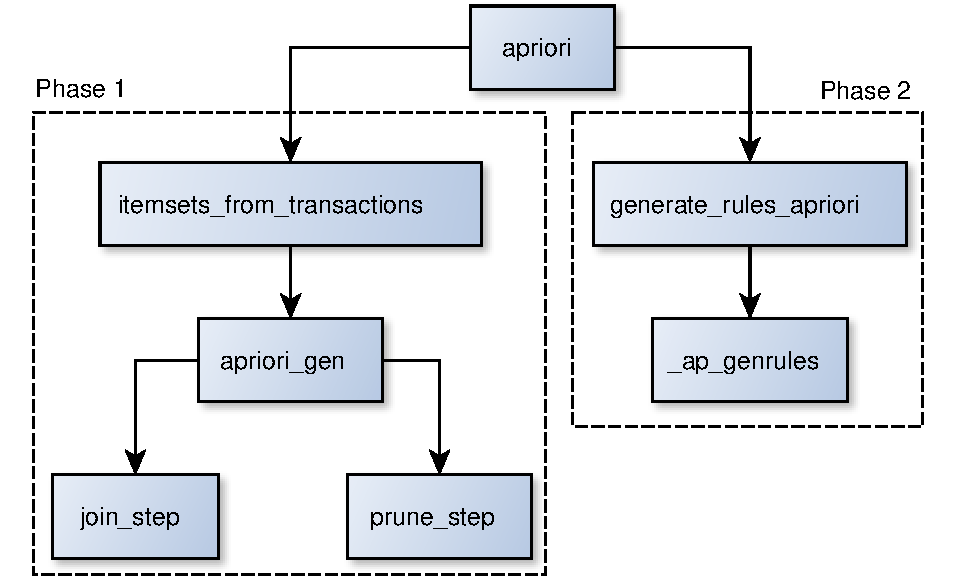
\includegraphics[width=12cm]{figs/apriori_software_functions.pdf}
	\end{center}
	{\footnotesize Software found at \url{https://github.com/tommyod/Efficient-Apriori}.}
\end{frame}

% -------------------------------------------------------------------------
\section{Summary and references}
\begin{frame}[fragile]{Summary and references}
	
	The Apriori algorithm discovers frequent itemsets in phase 1, and meaningful association rules in phase 2.
	Both phases employ clever bottom-up algorithms.
	By application of the downward closure property of itemsets (support) and rules (confidence), candidates may be pruned prior to expensive computations.
	
	\vfill
	
	\begin{easylist}[itemize]
		\ListProperties(Space=\listSpace, Space*=\listSpace)
		# The Python implementation ##
		 \href{https://github.com/tommyod/Efficient-Apriori/}{\texttt{github.com/tommyod/Efficient-Apriori}}
		
		# The original paper
		## Agrawal et al, \emph{Fast Algorithms for Mining Association Rules}, 1994  \url{http://www.cse.msu.edu/~cse960/Papers/MiningAssoc-AgrawalAS-VLDB94.pdf}
		
	\end{easylist}
\end{frame}

\end{document}